\section{Design Requirements}
\subsection{User Requirements} \label{sub:userRequirments}
\subsubsection{Introduction}
The project aims to develop a classroom management tool that works based on the theories discussed in the literature review chapter and also draws \emph{Adaptive User Interface} techniques to improve the users interaction with the systems interface. The following are what the user should require from the system. The requirements are given ranks.\footnote{ Mandatory :- the feature must be built into the final system; Desirable :- the feature must be built into the final system if time permits; Possible Enhancement :- the feature could be included as a future work} Table \ref{tab:user-requirements} contains a list of user requirements.






\begin{table}[htbp]
\begin{tabular}{|L|c|L|}\hline
Requirement & Rank & Description \\\hline
Account Registration & Mandatory &  \multicolumn{1}{m{8cm}|}{The systems interface provides a registration mechanism for new users to create an account. This mechanism requires the user to choose a password and email account that when validated would be used by the user for subsequent access to the system.}\\\hline
  Login & Mandatory & \multicolumn{1}{m{8cm}|}{This component forms part of the registration mechanism and it accepts the email address and password the user used in the registration process to authenticate the user and allow access to the system. } \\\hline
  Logout & Mandatory & \multicolumn{1}{m{8cm}|}{Users can log out of the system once they have been authenticated and are in the system. This provides them with a safe and secure way to leave the system and preserve the current state.} \\\hline
  Add class groups & Mandatory & \multicolumn{1}{m{8cm}|}{System interface will give users the feature to add new class groups to their workspace once they have been authenticated and granted access to the sytem. } \\\hline
Create seating arrangements & Mandatory & \multicolumn{1}{m{8cm}|}{The classroom component of the system's interface will provide a canvas for the user to create a seating plan in free form, \footnote{free form - denotes the canvas has no grid constraints and that the user can have any shape to the seating arrangements}. The classroom renders only thirty (30) cards, \footnote{cards represent pupils or students on the classroom space} as OFSTED \cite{OFSTED} states that is the optimal number of students any one teacher can effectively manage in a classroom.} \\\hline
 Upload pupil data & Mandatory & \multicolumn{1}{m{8cm}|}{The upload component can allow users to upload pupil data in a standard format,\footnote{Comma Separated Values (csv)} into the system.} \\\hline
  Save seating plans & Mandatory & \multicolumn{1}{m{8cm}|}{The history manager component of the user interface can save the current seating plan that the user is using at any point in time.} \\\hline
  Retrieve seating plans & Mandatory & \multicolumn{1}{m{8cm}|}{History manager component can also retrieve old seating plans or arrangements that relate to the user.} \\\hline
  Update seating plans & Mandatory & \multicolumn{1}{m{8cm}|}{As well as saving and retrieving, the history manager component can update old seating arrangements with the current arrangements on the canvas(classroom space).} \\\hline
  Scoring System & Mandatory & \multicolumn{1}{m{8cm}|}{The history item component provides a scoring feature that allows the user to score or rate the plans and or seating arrangements that they use.} \\\hline
  Delete year groups & Desirable & \multicolumn{1}{m{8cm}|}{The menu tab component of the system interface can delete the current year group selected by the user.} \\\hline
  Edit year group name & Desirable & \multicolumn{1}{m{8cm}|}{The menu tab component can also edit the name of the currently selected year group by the user.} \\\hline
  Delete class group & Desirable & \multicolumn{1}{m{8cm}|}{The menu item component can delete the currently selected class. } \\\hline
  Edit class group name & Desirable & \multicolumn{1}{m{8cm}|}{The menu item component can edit the name of the currently selected class.} \\\hline
  Delete old seating arrangements  & Desirable & \multicolumn{1}{m{8cm}|}{The history manager can delete old seating arrangements that are of no relevance to the user.} \\\hline
  Google Spreadsheet Integration & Possible Enhancement & \multicolumn{1}{m{8cm}|}{The upload can upload pupil data from google spreadsheet application programming interface if the user has pupil data located on the google spreadsheet system.
} \\\hline
  Report Generation & Possible Enhancement & \multicolumn{1}{m{8cm}|}{The information component can generate reports on best or optimal seating arrangements used by the user.} \\\hline
  one & two & \multicolumn{1}{m{8cm}|}{} \\\hline
\end{tabular}
\caption{\label{tab:user-requirements}User requirements table}
\end{table}

\subsection{Functional Requirements}
The system interface must provide components that allows the following functionalities.
\subsubsection{Authentication}
The user interface of the system must authenticate the user on registration and on logging in.

\textbf{Rationale} - This provides security and restricts access to system data and also allows the system to tailor its features and functionalities to the user based on their unique session ids.

\subsubsection{Account Creation}
The system must allow new users to the system to create their own accounts.

\textbf{Rationale} - This is the only mechanism through which potential users can obtain access to the system.

\subsubsection{Log in to user account}
The system must provide users the ability to sign into their account, if they are returning users.

\textbf{Rationale} - Users need to be able to return to use the system.

\subsubsection{Log out of user account}
The system must provide users with the ability to log out of the system.

\textbf{Rationale} - This allows the system to safely save the users state and protect the users data by protecting against unauthenticated access.

\subsubsection{New class groups}
The system must allow both new and old users to add new class groups to their workspace.

\textbf{Rationale} - Users are more likely to teach more than one class.

\subsubsection{CRUD Seating Arrangements}
The system must provide users the ability to CRUD\footnote{Create, Update, Delete} seating arrangements or plans on the user interface.This feature must be adaptive in that, it should alter seating rules to suit the preferences of the user.

\textbf{Rationale} - This is the core functionality of the system, the system would not be a classroom management tool if it lacked the ability to perform seating arrangements.

\subsection{Non-Functional Requirements}
\subsubsection{Overview}
The previous section laid more emphasis on what our system should do in order to achieve its aims and objectives, we briefly explained each functionality and the rationale behind it. In this section we will highlight the overall properties of the system, by specifying the standards that can be used to form an opinion of the overall operation of the system. The project is mainly concerned with the user interface features and functionality and as a result uses Firebase\cite{website:Firebase}, a platform that provides infrastructure and backend as a service. The use of Firebase makes it possible to provide requirements such as security and data integrity out of the box, allowing the project to focus on its main purpose and that is to create an adaptive user interface for a classroom management tool.

\subsubsection{Adaptivity}
The system shall provide adaptivity by restructuring its interface to reflect the most relevant features to the user. 

\subsubsection{Security}
The system shall be secure by only giving direct access to the system and its features to authenticated users. The authentication is provided by a trusted third-party solution, Firebase \cite{website:Firebase}. The encryption and security features provided by Firebase shall make the account registration, log in and logout operations of the system meet the security requirement.

\subsubsection{Data Integrity}
Firebase also provides real-time database management API\footnote{Application Programming Interface}. The accuracy of user data submitted to the system are consistently stored through this process. This features ties in with the security features by providing access control and data validation, example all emails and passwords used in registration are all validated before the process is complete. The upload component of the system also validates all pupil data uploaded to make sure they are in the required document format.\footnote{the use of format here refers to CSV}

\subsubsection{Usability}
The purpose of the project revolves around the ease of use of a classroom management tool. The system shall provide an interface that improves on its interaction with the user and has clarity in this interaction. It takes 3 steps for the user to go from a new user to a classroom with pupil data and seating plan, recording 5 clicks in the process. A returning user can create a new classroom with pupil data all in one step, subject to the information the system will have about him or her. These steps are all clear and on a clean user interface. 

\subsubsection{Reliability}
The system shall provide reliability with regards to its ability to perform required functions.Data storage and retrieval, access control are provided by a state of the art system that is Firebase. The systems clean user interface shall be reliable in creating a classroom space and suggesting the optimal seating arrangement for the user.The metric to measure our systems reliability is the consistency with which it presents contents\footnote{Content in this context refers to classes, year groups and pupil or student data} 

\subsubsection{Performance}
Performance with regards to this project is concerned with the interfaces reaction to how the user uses the system and how it makes recommendations to the user. The system shall start monitoring the user immediately after the sign up process and resume on subsequent sign ins. Our systems performance is measure by the time it takes to render pupils in the classroom with the required colour outline as per the adaptation rule.

\section{System Design}

\subsection{Overview}
The previous section detailed standards of measurement of our system as a requirement; we looked at each requirement and how our system meets each requirement. The following section discusses the thought process behind the design of our system.

\subsection{High level design}
Controllability, predictability and transparency are some of the important influences in designing effective systems \cite{hook1995glass}. \cite{rudisill1996human} maintains that the user should enjoy using the system. These factors were taken into consideration during the designing of the system. We attempt to improve the user's experience rather than substitute them. At a high level figure \ref{fig:SystemDesign} below reflects these guidelines in our system design.

\begin{figure}[!ht]
\caption{System Design}
    \label{fig:SystemDesign}
    \centering
    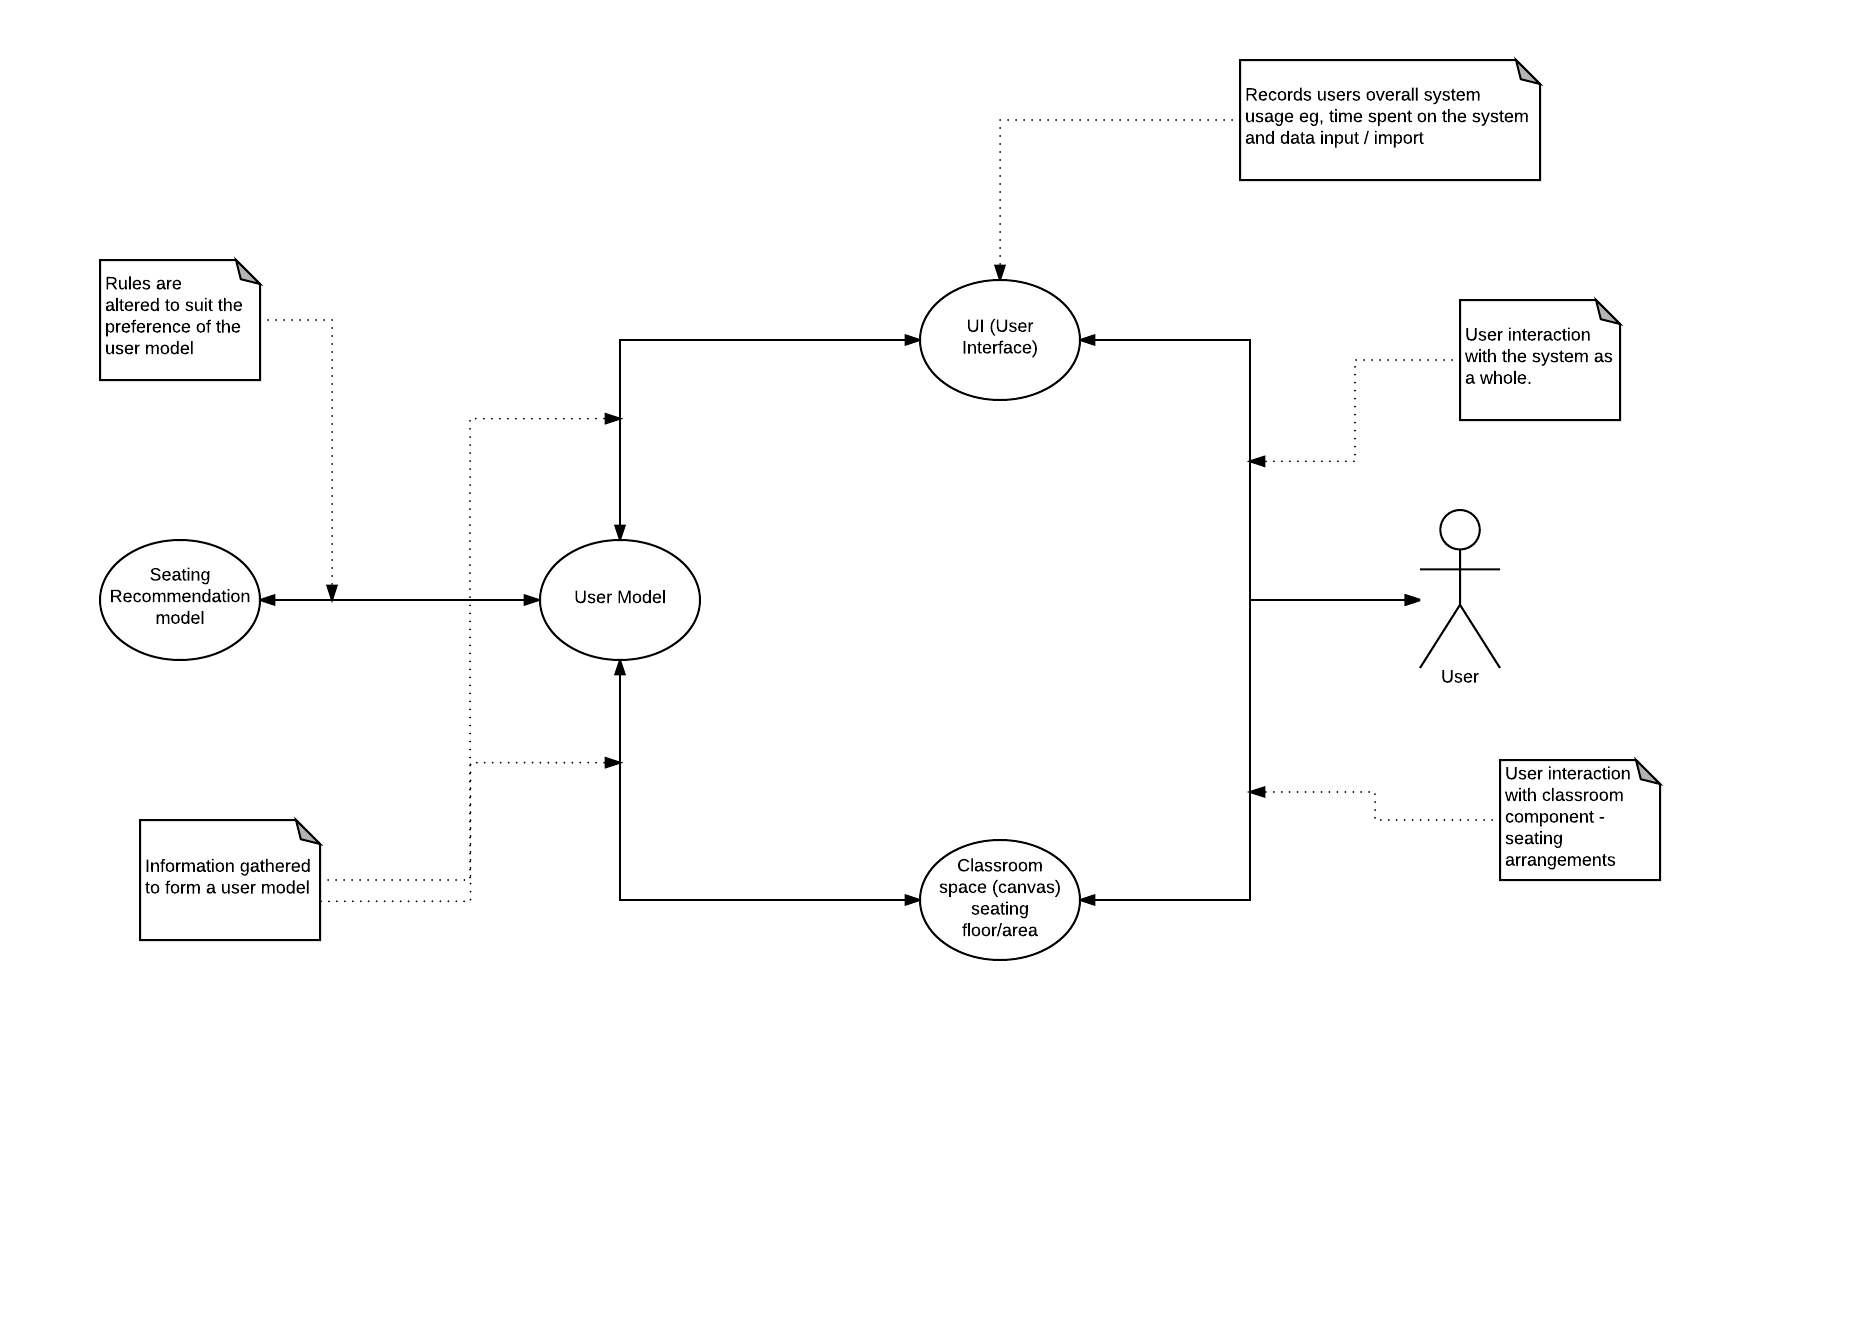
\includegraphics[scale=0.5]{figures/SystemDesign}
\end{figure}


The user of our system mainly interacts with the UI(User Interface) performing all relevant actions and steps, the UI contains the classroom area but the component responsible for the functionality operates in isolation much like all the other components in that it gathers information from the user that the general UI component does not have access to. Example the seating arrangement currently on the canvas(seating floor). A \emph{User Model} is created out of the information gathered by these components.

\subsection{User Model} \label{sub:UserModel}
The principal purpose of adaptation is to offer a simple, powerful and efficient interface to the user. We will be developing a system that offers such an interface by using the \emph{User Model} approach. By definition a \emph{User Model} is a representation of the knowledge and preferences of the user, these representations are depicted in the form of variables in the system. At the lower-level the user model is indeed an algorithm that creates an object with rules, the rules are then interpreted at the UI level to a user profile.

\subsection{User Interface}
Creating an interface with complete autonomy comes at a cost, as it affects the usability of the whole system.  We take the \emph{User Model} approach as it will not reduce the usability of the system. \emph{User Model} allows us to be able to identify tasks that we can assist the user in, by performing user analysis. \emph{User Analysis} comprises what the user needs to do in the system and what the user will do with the system.

We will only adapt :
\begin{itemize}
    \item the system where users are least adaptable,
    \item to features which have the largest impact on interaction,
    \item to the needs of intermittent and discretionary users. \cite{benyon1993adaptive} 
\end{itemize}

We can achieve this through a \emph{User Model} because we have a representation of the users and their interaction with the system, we can alter the interface without costing the user clarity in interaction.


\subsection{User Modeling}
User Modeling is the process of obtaining information about the user, this can done in numerous ways but we gather information:
\begin{itemize}
    \item  implicitly,
    \item  explicitly.
\end{itemize}

\textbf{Explicit Collection} - We gather information about the user explicitly through the registration form, settings form, login form and the seating arrangement scoring card. These are explicit as we ask the user for information such as the subject they teach, menu layout and their best seating arrangements.

\textbf{Implicit Collection} - We also gather information implicitly through the forms, information such as when the user logs in and when they logged out to infer the time spent on the system. How often they toggle(open and close) the menu tray and also make computations based on their highest scoring seating arrangements to determine the adaptation rule to apply when recommending seating arrangements to the user.\ref{fig:User-Model}

The system is designed to adapt its rules, that is, what it perceives to be the best and optimal seating plan to suit or match what the user actually perceives to be the best and optimal seating.We adopt this format of adaptation because the theories backing classroom management are not fool-proof and that what the theories suggests could be completely wrong for a particular classroom and teacher.

\subsection{Classroom Canvas} \label{sub:classroom}
The classroom canvas is used to create and update seating plans. This is where the rendering of pupils and their seating positions is performed, the classroom component has an instance of the \emph{recommendation object}. The seating patterns are recorded and stored by the \emph{history manager} component responsible for storing, retrieving and updating seating plans. The recommendation is initiated when the user starts to manipulate pupil seating positions on the canvas. A green outline on the pupil card suggests the pupil is paired or put in the best position as suggested by the rules currently being applied. A red outline suggests the position or pairing is not optimal. The user can of course ignore this - the plan they save as a result can be considered as an optimal plan or arrangement if they score it above 4 points. Each seating arranged store by the manager is given a score out of 5. The scoring is at the discretion of the user.

\subsection{Recommendation Model} \label{sub:RM}
The recommendation model is an algorithm that recommends optimal seating arrangements based on the user model (specifically the highest rated seating arrangements), by analysing the user model and proposing an adaptation rule that reflects the seating arrangement preferences of the user. 

\subsection{Web Workers} \label{sub:webworkers}
The core components of our system are the User and Recommendation Models; these have been designed to work in the background thread as web workers so as to not slow down the rendering of the user interface whiles these models perform computations. ``Web Workers are a mechanism by which a script operation can be made to run in a background thread separate from the main execution thread of a web application. The advantage of this is that laborious processing can be performed in a separate thread, allowing the main (usually the UI) thread to run without being blocked/slowed down''.\cite{website:Mozilla-WebWorkers}
\section{System Architecture}
\subsubsection{Overview}
In the previous section we looked at and briefly described the main design elements or components that make up the system.This section introduces the architectural style used to implement our system. 
\subsection{Architecture}
Our system uses a 2 tier system architecture, a presentation layer comprising the user interface and a resource layer (server) provided by Firebase \cite{website:Firebase}. Firebase facades all the details of a server, database and security from the project so we are able to focus primarily on the presentation layer (User Interface). The figure below illustrates the top level architecture of the system. We adopt a plug and play (component architecture) architectural style. 
\begin{figure}[!ht]
\caption{System Architecture - Top Level}
    \label{fig:SystemArchitecture}
    \centering
    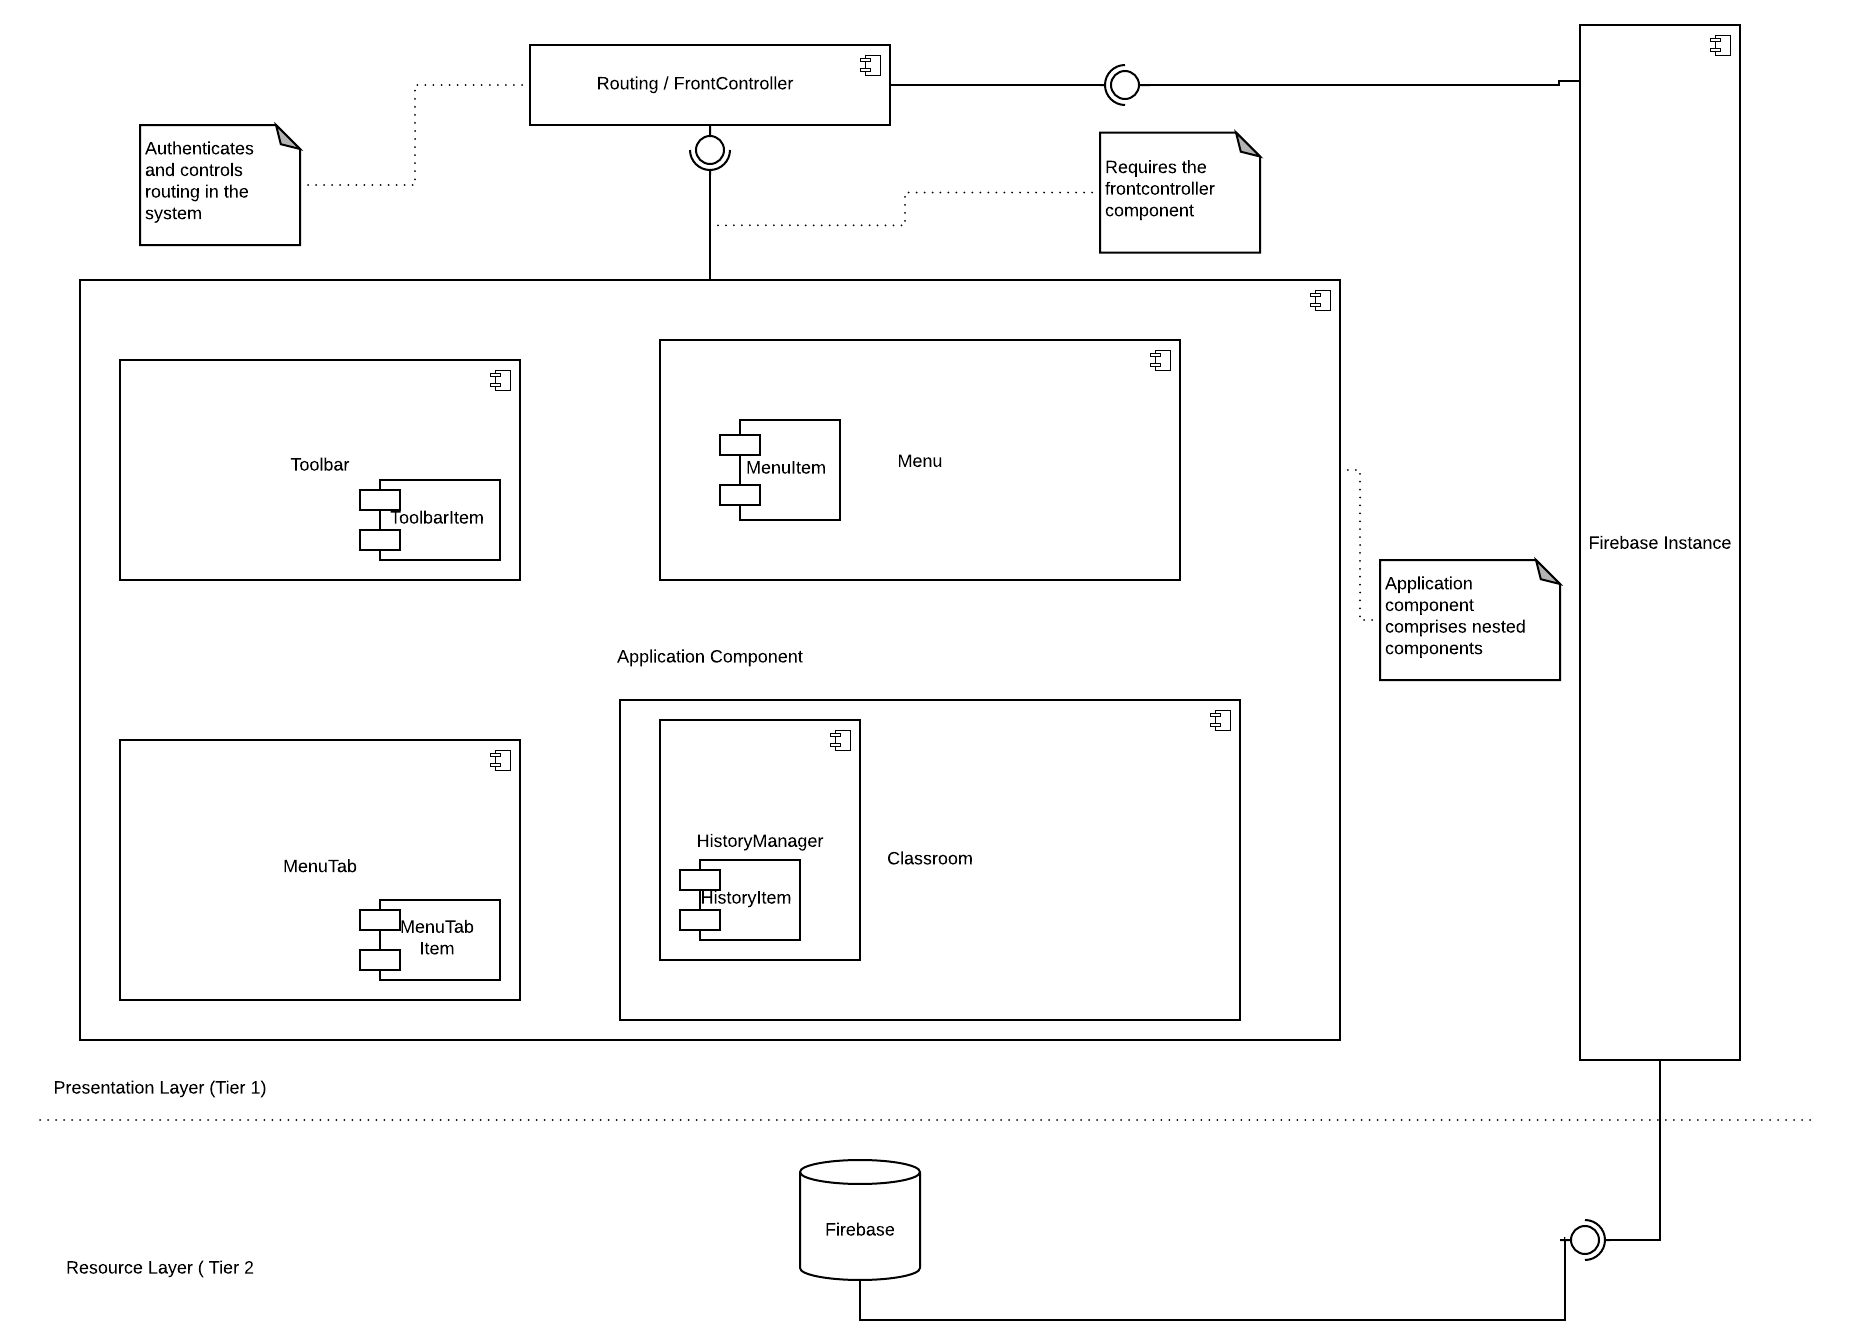
\includegraphics[scale=0.5]{figures/SystemArch}
\end{figure}
Figure \ref{fig:SystemArchitecture} below shows the main components that make up our system in their respective layers.
\subsubsection{Front controller}
The front controller provides our system with a single point of entry to handle requests and provides navigation from one component view to the other as the user performs tasks in our system. Our system is concerned with the User Interface therefore a simple and lightweight architecture and design patterns such as this suits our aim and objectives with the project.

\subsubsection{Firebase Instance}
A firebase instance is used as a proxy to make API calls to Firebase over the internet. This component is responsible for security, data integrity and overall database management.

\subsubsection{Toolbar}
The toolbar component is responsible for creating and presenting toolbar items such as the login and logout items.Each toolbar item is an instance of another component called ``toolbarItem''.

\subsubsection{Menu}
The menu mainly comprises the list of classes available to the user. The menu component is responsible for retrieval and displaying the correct list of classes pertaining to a specific user in our system.

\subsubsection{MenuTab}
In the header section of our system we display the year groups. Year groups are the age range of the pupil in the classes that the teacher teaches. These year groups are retrieved and display by the MenuTab component, as ``MenuTabItems''.

\subsubsection{Classroom}
The classroom component comprises a canvas on which seating arrangements are rendered as described in \ref{sub:classroom}. 
\subsubsection{History Manager} \label{sub:historyManager}
This component as the name implies holds references to all seating arrangements saved by the user in the system, each reference is an instance of another component called ``historyItem''. 

\subsection{Component Architecture}
In the overview sub section of this section we mentioned \emph{Plug and play architectural} style, each functionality in our system is provided by a component that operates in isolation. This makes it possible for us to remove a component and replace it with another. \cite{clemens1998component} defines a component as a unit of composition with contractually specified interfaces and explicit context dependencies, a software component can be deployed independently and is subject to third part composition.
\subsubsection{Web components}
Our components are developed based on the \emph{Web Components}\footnote{ Web component in our system is based on PolymerJS framework} standards. \cite{website:Mozilla-Developer}. A web component is a reusable interface widget that is created with open web technologies. \footnote{Open web technologies like standard HTML elements} 